\chapter{Metric Spaces}
\section{Fundamentals}
\begin{defn}
Let $X$ be a set. A \vc{metric} on $X$ is a function $d:X\times X\rightarrow [0,\infty)$ that satisfies: 
\begin{enumerate}
\item[(a)] $d(x,y)=d(y,x)$ for any $x,y\in X$
\item[(b)] $d(x,y)\leq d(x,z)+d(z,y)$ for any $x,y,z\in X$
\item[(c)] $d(x,y)=0$ iff $x=y$
\end{enumerate}
If a function $d$ satisfies (a), (b) above, and $d(x,x)=0$ for all $x\in X,$ then $d$ is a \vc{semi-metric}.
\end{defn}

\Ex On $\C{n},$ the following are common metrics:
\begin{itemize}
\item $d_p(v,w)=\Big(\sum\limits_{j=1}^n |v_j-w_j|^p\Big)^{1/p}$ for $p\geq 1$
\item $d_{\infty}(v,w)=\sup\{|v_j-w_j|:1\leq j\leq n\}$
\end{itemize}
(Verify that these are metrics.) \\ \\
Fact: If $S\subseteq X,$ and $d$ is a metric on $X,$ then $d$ is a metric on $S.$ \\

\begin{defn} 
Let $V$ be a vector space over $\R{ }$ or $\C{ }.$ A \vc{norm} on $V$ is a function $\norm{\cdot}:V\rightarrow[0,\infty)$ such that:
\begin{enumerate}
\item[(a)] $\norm{cv}=|c|\cdot\norm{v}$ for $c\in \R{}$ or $\C{}$ and $v\in V$
\item[(b)] $\norm{v+w}\leq\norm{v}+\norm{w}$ for $v,w\in V$
\item[(c)] $\norm{v}=0$ implies $v=0$
\end{enumerate}
A function that satisfies only (a) and (b) above is called a \vc{seminorm}.
\end{defn}

\noindent Remark: Any norm $\norm{\cdot}$ on $X$ induces the metric $d(x,y):=\norm{x-y}.$ \\ \\ \\
\Ex Let $V$ be the space of continuous functions on $[0,1].$ Then  \\ $\norm{f}_{\infty}=\sup\{|f(x)|:x\in[0,1]\}$ is a norm on $V.$ \\
It can also be shown that $\norm{f}_p:=\Big(\int_0^1 |f(x)|^p\;dx\Big)^{1/p}$ is a norm on $V.$ \\

\begin{defn}
Let $(X,d_x)$ and $(Y,d_y)$ be metric spaces. A function $f:X\rightarrow Y$ is \vc{isometric} if $d_y(f(v),f(w))=d_x(v,w)$ for all $v,w\in X.$
\end{defn}
\begin{itemize}
\item Note that all isometries are injective.
\end{itemize}

\noindent\Ex If $S\subseteq X,$ and $f:S\rightarrow X$ is defined by $f(x)=x$ (inclusion), then $f$ is an isometry. \\ \\
If $f$ is onto, then $f$ is viewed as an isomorphism between $(X,d_x)$ and $(Y,d_y).$ $f^{-1}$ is also an isomorphism.
\begin{defn} 
A function $f:X\rightarrow Y$ is \vc{Lipschitz} if there is a constant $k\geq 0$ such that $d_y(f(x_1),f(x_2))\leq k\cdot d_x(x_1,x_2).$ The smallest such constant is the \vc{Lipschitz constant} for $f.$
\end{defn}

\begin{defn} 
$f:X\rightarrow Y$ is \vc{uniformly continuous} if for any $\epsilon>0,$ there exists $\delta>0$ such that $d_y(f(x_1),f(x_2))<\epsilon$ whenever $d_x(x_1,x_2)<\delta.$
\end{defn}
\begin{itemize}
\item It is easy to see that if $f$ is Lipschitz, then it is uniformly continuous.
\end{itemize}

\begin{defn} 
$f:X\rightarrow Y$ is \vc{continuous at $x_0$} if for any $\epsilon>0,$ there exists $\delta>0$ such that $d_y(f(x),f(x_0))<\epsilon$ whenever $d_x(x,x_0)<\delta.$ We say $f$ is \vc{continuous} if it is continuous at every $x\in X.$
\end{defn}

\begin{defn} 
A sequence $\{x_n\}$ in $X$ \vc{converges} to $x^*\in X$ if for any $\epsilon>0,$ there exists $N\in\mathbb{N}$ such that for all $n\geq N,$ we have $d(x_n,x^*)<\epsilon.$
\end{defn}

\begin{prop} 
A function $f:X\rightarrow Y$ is continuous iff $x_n\rightarrow x$ implies $f(x_n)\rightarrow f(x).$ \\ \\
\pf{\textit{Exercise.}}
\end{prop}

\begin{defn}
$S\subseteq X$ is \vc{dense} in $X$ if for any $x\in X$ and $\epsilon>0,$ there exists $s\in S$ such that $d(x,s)<\epsilon.$
\end{defn}

\begin{prop}
Let $S$ be dense in $X,$ and let $f:X\rightarrow Y$ and $g:X\rightarrow Y$ be continuous functions such that $f(s)=g(s)$ for all $s\in S.$ Then $f=g$ on $X.$ \\ \\
\pf{Let $x\in X\setminus S,$ and let $\epsilon>0.$ Then there exists $\delta>0$ and $s\in S$ such that $d(f(x),f(s))<\epsilon/2,$ and $d(g(x),g(s))<\epsilon/2$ for $d(x,s)<\delta,$ by continuity and density. Then 
$$d(f(x),g(x))\leq d(f(x),f(s))+d(g(s),g(x))<\epsilon/2+\epsilon/2=\epsilon,$$
since $f(s)=g(s).$ Thus $d(f(x),g(x))=0,$ so $f(x)=g(x).$}
\end{prop}

\begin{defn}
A sequence $\{x_n\}$ is \vc{Cauchy} if for any $\epsilon>0,$ there exists $N\in\mathbb{N}$ such that $n,m\geq N$ implies $d(x_n,x_m)<\epsilon.$ \\
A metric space in which every Cauchy sequence converges is \vc{complete}.
\end{defn}

\noindent\Ex Consider $(\mathbb{Q}, |\cdot|).$ We know there exists a Cauchy sequence converging to $\sqrt{2}\in\mathbb{R},$ but in this metric space, $\sqrt{2}$ is not an element, so this sequence does not converge, hence this metric space is not complete.

\section{Completion of a Metric Space}

\begin{prop}
If $f:X\rightarrow Y$ is uniformly continuous, and $\{x_n\}$ is Cauchy in $X,$ then $\{f(x_n)\}$ is Cauchy in $Y.$ \\ \\
\pf{\textit{Exercise.}}
\end{prop}

\begin{defn}
Let $(X,d)$ be a metric space. A complete metric space $(\overline{X},\overline{d}),$ together with an isometric function $f:X\rightarrow\overline{X}$ with dense range is a \vc{completion} of $(X,d).$
\end{defn}
\begin{itemize}
\item Remark: Completions are unique up to isomorphism.
\end{itemize}

\begin{prop}
If $((Y_1, d_1), f_1)$ and $((Y_2,d_2),f_2)$ are completions of $(X,d),$ then there exists an onto isometry (metric space isomorphism) $g:Y_1\rightarrow Y_2$ with $f_2=g\circ f_1.$ This can be visualized by the following commutative diagram: \\
\begin{center}
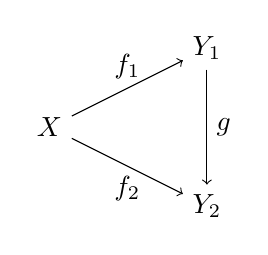
\begin{tikzpicture}
\node (a) at (0,0) {$X$};
\node (b) at (2,1) {$Y_1$};
\node (c) at (2,-1) {$Y_2$};
\draw[->] (a) -> (b) node[midway,above] {$f_1$};
\draw[->] (a) -> (c) node[midway,below] {$f_2$};
\draw[->] (b) -> (c) node[midway,right] {$g$};
\end{tikzpicture}
\end{center}
\end{prop}

\noindent Every metric space has a completion, and the proof will be constructive. The completion will be defined using equivalence classes of Cauchy sequences. We will need the following lemmas to support the construction.

\begin{frame*}
\noindent \ub{Lemma 1}: If $\{s_n\}$ and $\{t_n\}$ are Cauchy sequences in $X,$ then the sequence $\{d(s_n,t_n)\}$ in $\R{}$ converges. \\
\pf{\textit{Exercise. Hint:} $\{d(s_n,t_n)\}$ is a Cauchy sequence in a complete metric space.}
\end{frame*}

\begin{frame*}
\noindent \ub{Lemma 2}: Let $\text{Cau}(X)$ denote the set of all Cauchy sequences in $X.$ Then the relation $\{s_n\}\sim \{t_n\}$ iff $d(s_n,t_n)\rightarrow 0$ is an equivalence relation. \\ \\
\pf{Reflexivity and symmetry are trivial. Suppose $d(s_n,r_n)\rightarrow 0$ and $d(r_n,t_n)\rightarrow 0.$ Then $d(s_n,t_n)\leq d(s_n,r_n)+d(r_n,t_n)$ for all $n\in\mathbb{N}.$ The result follows immediately.}
\end{frame*}

\begin{frame*}
\noindent \ub{Lemma 3}: Let $\overline{X}$ be the set of all equivalence classes of $\text{Cau}(X)$ under the equivalence relation above. Then $\overline{d}:\overline{X}\rightarrow[0,\infty)$ defined by $\overline{d}(\{s_n\},\{t_n\}):=\lim\limits_{n\rightarrow\infty} d(s_n,t_n)$ is a metric on $\overline{X}.$ \\ \\
\pf{First, note that by Lemma 1, $\overline{d}$ is always defined. Since we are dealing with equivalence classes, we must show that $\overline{d}$ is also well-defined. Let $\xi,\eta\in\overline{X},$ and let $\{x_n\},\{s_n\}\in\xi,$ and $\{y_n\},\{t_n\}\in\eta.$ We have $\lim d(x_n,s_n)=\lim d(y_n,t_n)=0.$ Thus, \\ $d(s_n,t_n)\leq d(s_n,x_n)+d(x_n,y_n)+d(y_n,t_n).$ For any $\epsilon>0,$ we can find $N\in\mathbb{N}$ such that both $d(s_n,x_n)<\epsilon/2$ and $d(y_n,t_n)<\epsilon/2$ for $n\geq N.$ Then $|d(s_n,t_n)-d(x_n,y_n)|<\epsilon.$ It follows that $\overline{d}(\xi,\eta)=\lim d(x_n,y_n)=\lim d(s_n, t_n),$ so that $\overline{d}$ is indeed well-defined. \\  \\
Symmetry is trivial. The triangle inequality follows from the proof to Lemma 2. If $\overline{d}(\xi,\eta)=0,$ then for any $\{x_n\}\in\xi, \{y_n\}\in\eta,$ we have $\lim d(x_n,y_n)=0,$ so in particular, $\{y_n\}\in\xi,$ hence $\xi=\eta.$}
\end{frame*}

\begin{thm}
Let $(X,d_x)$ and $(Y,d_y)$ be metric spaces with $Y$ complete. If $S\subseteq X$ is dense, and $f:S\rightarrow Y$ is uniformly continuous, then there exists a unique continuous extension $\overline{f}:X\rightarrow Y$ of $f.$ In fact, $\overline{f}$ is uniformly continuous. \\ \\
\pf{(Existence only) For $x\in X,$ choose a Cauchy sequence $\{s_n\}$ in $S$ converging to $x.$ Then $\{f(s_n)\}$ is Cauchy in $Y,$ so it converges to a point $p\in Y.$ Set $\overline{f}(x):=p.$ We show that $\overline{f}$ is well-defined. Indeed, if $\{t_n\}\in\text{Cau}(S)$ and converges to $x,$ then we have $\lim d_x(s_n,t_n)=0,$ implying that $\lim d_y(f(s_n),f(t_n))=0.$ Therefore $\lim d_y(f(t_n),p)=0,$ so $\{f(t_n)\}$ converges to $p$ also. It remains to show continuity, which is left as an exercise.}
\end{thm}

\begin{thm}
Every metric space $(X,d)$ has a completion. \\ \\
\pf{As in Lemma 3, $(\overline{X},\overline{d})$ is a completion of $(X,d).$ We embed $X$ in $\overline{X}$ by the isometry $\iota:X\rightarrow\overline{X}$ defined by $\iota(x):= [\{x,x,x,...\}],$ where $[\cdot]$ denotes the corresponding equivalence class. Note that $\overline{d}\Big|_X=d,$ i.e., $\overline{d}(\iota(x),\iota(y))=d(x,y).$\\ It remains to show that $\overline{d}$ has dense range, and that $(\overline{X},\overline{d})$ is complete.
\begin{itemize}
\item Let $\xi\in\overline{X}, \epsilon>0, \{x_n\}\in\xi.$ There exists $N\in\mathbb{N}$ such that $n,m\geq N$ implies $d(x_n,x_m)<\epsilon.$ Then $\overline{d}(\iota(x_N),\xi)=\lim\limits_{n\rightarrow\infty} d(x_N,x_n)<\epsilon.$ Therefore $\overline{d}$ has dense range by considering $\iota(x_N).$
\item Let $\{\xi_n\}$ be a Cauchy sequence in $\overline{X}.$ For each $m\in\mathbb{N},$ pick $x_m\in X$ such that $\overline{d}(\iota(x_m),\xi_m)<1/m.$ Then $\{x_m\}$ is a Cauchy sequence, and it follows that $\{\xi_m\}$ converges to the equivalence class of $\{x_m\}.$
\end{itemize}}
\end{thm}

\noindent Remark on functions:\\
Denote $C([0,1])$ the space of continuous functions on $[0,1].$ Consider the metric space $C([0,1])$ induced by the norms $\norm{\cdot}_{\infty}$ or $\norm{\cdot}_p.$ This space is not complete. It is easy to come up with a sequence of continuous functions converging under these norms to a function that is not continuous. \\

\noindent Vector Space Remark: \\
Let $V$ be a vector space with norm $\norm{\cdot}.$ Consider $V^{\infty},$ the space of all sequences of elements in $V.$ This is also a vector space. It can be shown that $\text{Cau}(V)$ is a subspace of $V^{\infty}.$ \\
Now let $\mathcal{N}(V)$ denote the set of all Cauchy sequences in $V$ converging to $0.$ Then $\mathcal{N}(V)$ is a subspace of $\text{Cau}(V).$ If $\{v_n\}$ and $\{w_n\}$ are equivalent Cauchy sequences, then \\ $\norm{v_n-w_m}\rightarrow 0,$ so $\{v_n-w_n\}\in\mathcal{N}(V).$ Thus $\overline{V}$ is in fact the quotient space $\text{Cau}(V)/\mathcal{N}(V).$ \\ \\
Fact: Any two norms $\norm{\cdot}_1,\norm{\cdot}_2$ on a finite dimensional vector space are \ub{equivalent}, meaning that there are constants $c,C>0$ such that $c\norm{x}_1\leq\norm{x}_2\leq C\norm{x}_1$ for all $x.$ If a function is continuous with respect to a particular norm, then it is easily seen that it is continuous with respect to any equivalent norm.

\section{Openness}

\begin{defn}
If $(X,d)$ is a metric space, the \ub{open ball} of radius $r$ around $x$ is \\ $B_r(x):=\{y\in X: d(x,y)<r\}.$
\end{defn}

\begin{defn}
We can rephrase continuity as $f:X\rightarrow Y$ is continuous at $x_0$ if for any $\epsilon>0,$ there exists $\delta>0$ such that $f\Big(B_{\delta}(x_0)\Big)\subseteq B_{\epsilon}(f(x_0)).$
\end{defn}

\noindent
If $y\in B_{\epsilon}(f(x_0))$ and $y=f(x)$ for some $x\in X,$ let $\epsilon'=\epsilon-d(y,f(x_0))>0.$ Then $B_{\epsilon'}(y)\subseteq B_{\epsilon}(f(x_0)),$ so there exists $\delta'>0$ such that $f\Big(B_{\delta'}(x)\Big)\subseteq B_{\epsilon}(f(x_0)).$ \\
If $x_1\in f^{-1}\Big(B_{\epsilon}(f(x))\Big),$ there is an open ball $B_{\delta'}(x)$ such that $B_{\delta'}(x_1)\subseteq f^{-1}\Big(B_{\epsilon}(f(x))\Big).$ Thus $f^{-1}\Big(B_{\epsilon}(f(x))\Big)$ is a union of open balls in $X.$ Similarly, $f^{-1}(B_{\epsilon}(y))$ is a union of open balls in $X.$

\begin{defn}
A subset $\mathcal{O}\subseteq X$ (where $X$ is a metric space) is \ub{open} if it is a union of open balls in $X.$
\end{defn}

By the arguments above, it can be shown that $f:X\rightarrow Y$ is continuous iff for any open ball $B_{\epsilon}(y)\subseteq Y,$ we have that $f^{-1}(B_{\epsilon}(y))$ is open in $X.$ \\

\noindent Set theoretic facts:\\
Let $f:X\rightarrow Y$ be a function, and let $\{A_{\alpha}\}$ be a family of subsets of $X.$ Then:
\begin{itemize}
\item $f^{-1}\Big(\bigcup_{\alpha} A_{\alpha}\Big) = \bigcup_{\alpha} f^{-1}(A_{\alpha})$
\item $f^{-1}\Big(\bigcap_{\alpha} A_{\alpha}\Big) = \bigcap_{\alpha} f^{-1}(A_{\alpha})$
\item $f^{-1}\Big(A_1\setminus A_2) = f^{-1}(A_1)\setminus f^{-1}(A_2)$
\item $f\Big(\bigcup_{\alpha} A_{\alpha}\Big) = \bigcup_{\alpha} f(A_{\alpha})$
\item $f\Big(\bigcap_{\alpha} A_{\alpha}\Big) \subseteq \bigcap_{\alpha} f(A_{\alpha})$
\item $f(A_1\setminus A_2)\supseteq f(A_1)\setminus f(A_2)$
\end{itemize}

\noindent Let $\mathcal{O}\subseteq Y$ be open. Then $f^{-1}(\mathcal{O})=f^{-1}\Big(\bigcup\limits_{U\subseteq\mathcal{O}, U\text{ open ball}} U\Big)=\bigcup\limits_{U\subseteq\mathcal{O}, U\text{ open ball}} f^{-1}(U).$ \\ Thus, if $f:X\rightarrow Y$ is continuous, and $\mathcal{O}$ is open in $Y,$ then $f^{-1}(\mathcal{O})$ is open in $X.$
\begin{thm}
If $(X,d)$ is a metric space, and $\tau_d$ is the collection of all open sets, then:
\begin{enumerate}
\item[(1)] If $\{\mathcal{O}_{\alpha}\}$ is an arbitrary collection of subsets in $\tau_d,$ then $\bigcup_{\alpha}\mathcal{O}_{\alpha}$ is open.
\item[(2)] If $\mathcal{O}_1,\hdots,\mathcal{O}_n$ is a finite collection of subsets in $\tau_d,$ then $\bigcap\limits_{j=1}^n \mathcal{O}_j$ is open.
\item[(3)] $X\in\tau_d$ ($X$ is open)
\end{enumerate}
\pf{
  \begin{enumerate}
  \item[(1)] Trivial
  \item[(2)] Let $x\in \bigcap\limits_{j=1}^n \mathcal{O}_j.$ For each $j,$ there exists $\delta_j>0$ such that $B_{\delta_j}(x)\subseteq\mathcal{O}_j.$ Let \\ $\delta=\min\{\delta_j:1\leq j\leq n\}.$ Then $B_{\delta}(x)\subseteq\mathcal{O}_j$ for each $j.$ This yields the desired result.
  \item[(3)] Let $\epsilon>0.$ Then $X=\bigcup\limits_{x\in X} B_{\epsilon}(x).$ The result follows from (1).
  \end{enumerate}
}
\end{thm}
\noindent By convention, $\varnothing\in\tau_d$ ($\varnothing$ is open).